\section{System Overview}
\label{sec:system_overview}

Figure \ref{fig:system} 
%shows the high-level architecture of 
gives an overview of the architecture of 
Qsearch that has been introduced in our earlier work \cite{HoISWC2019}. 
%The arrows in the figure depict information flow between the different system components. 
Qsearch consists of two main phases:
\textit{Extract}
and \textit{Answer}.
 
%In this section, we demonstrate our numerical question answering system from text. In Figure \ref{fig:system}, we present a high-level architecture of our system, where the arrows depict information flow between building blocks. We split the working flow of our system into two main stages: \textit{Extract} and \textit{Answer}.

\begin{figure}[t]
\centering
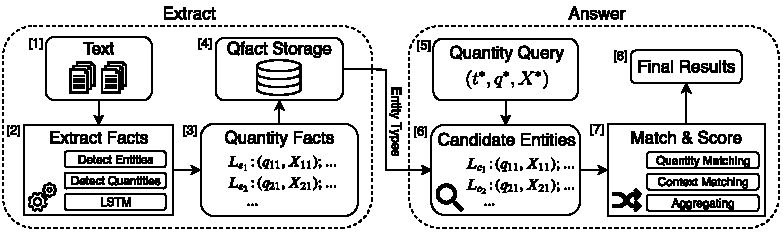
\includegraphics[width=0.5\textwidth]{figures/overview.pdf}
\caption{Overview of Qsearch \cite{HoISWC2019}.}
\label{fig:system}
\vspace{-1em}
\end{figure}
% what is the storage, how is it stored, and indexed 

\subsection{Extract}  
We preprocess to recognize named entities in the input text corpus (Block 1) using AIDA \cite{DBLP:conf/emnlp/HoffartYBFPSTTW11} system that links entity mentions
%in text are linked 
to the YAGO knowledge base \cite{DBLP:conf/www/SuchanekKW07}.
%and link them to an external knowledge base (KB).
%To achieve a better detection quality, we run NED on a per-document instead of per-sentence basis.
We also detect quantity mentions in the text and normalize them into standard units. For this, we make use of the Illinois Quantifier \cite{DBLP:journals/tacl/RoyVR15}, a state-of-the-art tool for 
recognizing quantities in text, along with some hand-crafted rules (e.g., regular expressions). 

Subsequently, we run a specifically designed Long Short Term Memory (LSTM) network to extract Qfacts in the form of triples $(e,q,X)$ from each individual preprocessed sentence (Block 2). The neural network structure has been described in our work \cite{HoISWC2019}. The main idea is that, for each quantity detected in the preprocessing step, the neural network identifies the entity to which it refers
and the relevant context tokens that express the relation between them. Figure \ref{fig:example} illustrates an example of how Qsearch extracts Qfacts from sentences. In this example, the quantity $q_1$ is mapped to the entity $e_1$ and context $\{\textit{price, Germany}\}$, whereas the quantity $q_2$ is also mapped to the entity $e_1$ but with context $\{\textit{range, battery}\}$.


After the neural-based extraction, all Qfacts having the same named entity are grouped together, so that each individual entity $e_i$ is connected with a list of quantities and contexts, expressed as $L_{e_i} = \{(q_{i1},X_{i1}),(q_{i2},X_{i2}),... \}$ (Block 3).
Entities are also linked to their semantic types from the KB, and we store these structures in a data repository in Block 4. In our implementation, Elasticsearch is used as the storage engine.

\begin{figure}[t]
\centering
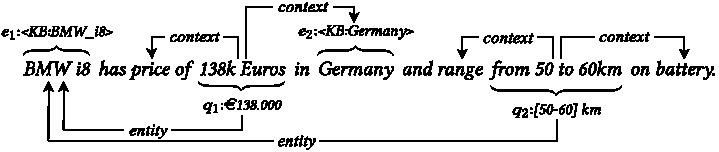
\includegraphics[width=0.5\textwidth]{figures/example_2.pdf}
\caption{Each detected quantity is linked to a corresponding entity and relevant context tokens.}
\label{fig:example}
\vspace{-1em}
\end{figure}

\subsection{Answer}
In this phase, Qqueries are answered by matching against Qfacts extracted from before. 

\noindent \textbf{Query Parsing.} In Block 5, the input questions are transformed into Qquery format $(t^*,q^*,X^*)$ by a rule-based parser. The parser uses a dictionary of YAGO types and a dictionary of quantity units to recognize the target semantic type of answers $t^*$ and the quantity condition $q^*$. Then, it includes all remaining tokens of the query (except stopwords) in the query context $X^*$ \cite{HoISWC2019}.

\noindent \textbf{Answer Matching.} First, based on the type information from the KB, a list of candidate entities $\mathcal{C} = \{c_1,c_2,...\}$ that satisfy the target type $t^*$ are retrieved from the Qfact repository, along with their quantity-context pairs $\{L_{c_1},L_{c_2},...\}$ (Block 6). Second, we perform quantity matching with the support of a list of unit conversion rules, filtering all Qfacts that do not meet the quantity condition $q^*$ (Block 7).
Finally, each candidate entity $c \in \mathcal{C}$ is assigned a score calculated based on matching contexts $X$ against $X^*$. 
%The candidate entities are ranked by their scores and returned to the user (Block 8).
Here, we make use of two context ranking models for measuring the context relevance: \textit{Kullback-Leibler divergence (KL)} and \textit{context embedding distance (ced)} (see \citep{HoISWC2019} for details).

 

%In the following Sections
%\ref{sec:extract} and \ref{sec:match}, we discuss in detail the
% Qfact extraction model and the matching and answering model, 
%respectively.

%In the remainder of this section, we discuss how each candidate entity is scored in Block 7.

\noindent \textbf{Kullback-Leibler Divergence.} The Kullback-Leibler divergence between the query context $X^*$ and the fact context $X$ is defined as:
\begin{align*}
\textit{KL}(X^*, X) &= H(X^*, X) - H(X^*) \\ &\equiv H(X^*, X) 
= -\sum_{w \in \mathcal{V}} P(w|X^*)\,\log P(w|X)
\end{align*}
where $\mathcal{V}$ is the word vocabulary, $H(X^*)$ is the entropy of $X^*$; $H(X^*, X)$ is the cross entropy between $X^*$ and $X$; and $\equiv$ is rank equivalence
(i.e., preserving order, $H(X^*)$ is omitted). 
%Since we are only interested in ranking fact contexts in response to a query context, we can omit $H(X^*)$.
The two probabilities $P(w|X^*)$ and $P(w|X)$ 
%for query context and fact context 
are estimated using Maximum Likelihood Estimation (MLE) with WordNet-based context expansion and Jelinek-Mercer smoothing to avoid zero probabilities \cite{HoISWC2019}.

% on an expanded version $X^*_E$ of $X^*$ as:
%\[P(w|X^*) = count(w \in X^*_E)/|X^*_E|\]
%To expand a query context, we resort to WordNet \cite{Miller:1995:WLD:219717.219748} and add all synonyms of the context words to it. For the fact context, we estimate the word probability $P(w|X)$ using Jelinek-Mercer smoothing 
%%to avoid zero probabilities
% as:
%\[P(w|X) = (1 - \lambda) \times count(w \in X)/|X| + \lambda \times P(w|B)\]
%This linearly combines the MLE from the fact context $X$ with the MLE obtained from a background corpus $B$. The smoothing parameter $\lambda$ (set to $\lambda=0.1$ in our system) controls the influence of the background corpus on the probability estimate. We construct the background corpus $B$ from all sentences of the entire text corpus that contain at least one quantity (total 39M sentences in our data). \\
%

%Since these two estimates are very sparse, before calculating, we expand $X^*$ and $X$ using an external resource. Moreover, a smoothing method is applied to avoid zero counts.
%\thinh{Should explain more? which resource, how to expand, which smoothing method.}

\begin{figure*}[t]
\centering
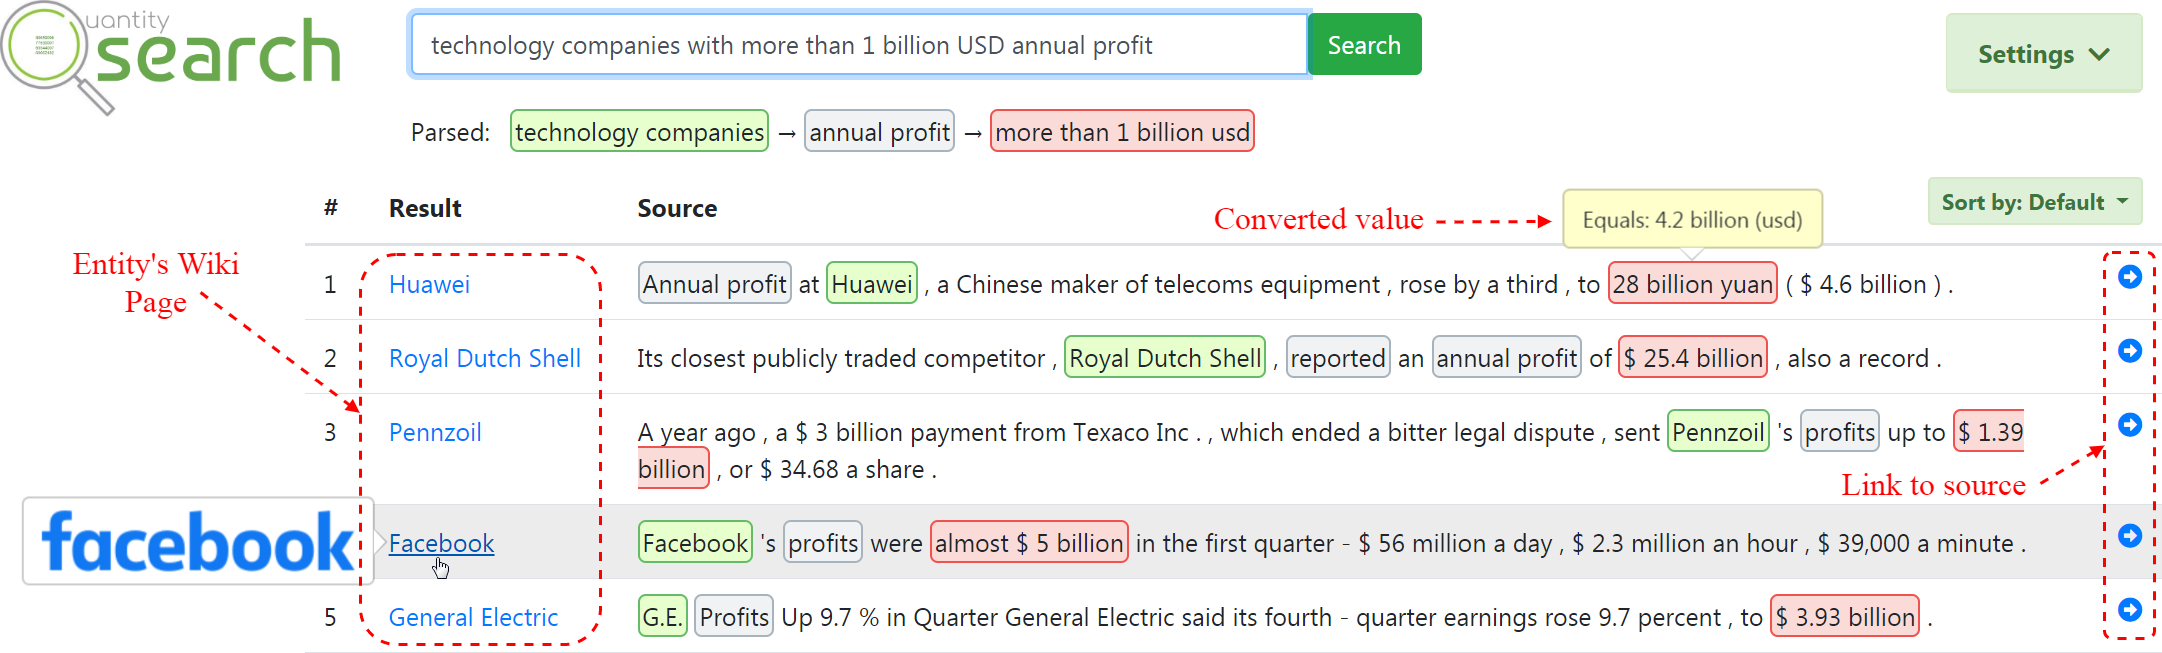
\includegraphics[width=1\textwidth]{figures/new/gui.png}
\caption{Qsearch Web interface.}
\label{fig:gui}
\vspace{-1em}
\end{figure*}

\noindent \textbf{Context Embedding Distance.}
The novel context embedding distance for measuring context relevance is defined as follows:
\[ced(X^*, X) = ded(X^* \rightarrow X) \times ded(X \rightarrow X^*)^\alpha\]
where $ded(A \rightarrow B)$ is the \textit{directed embedding distance} between two bags of words $A$ and $B$, computed as:
\[ded(A \rightarrow B) = 1 + \Bigg(\sum\limits_{u \in A} W(u)\min\limits_{v \in B}(d(u,v))\Bigg)\big/\sum\limits_{u \in A}W(u)\]
where $d(u,v)$ is the semantic distance between two words $u$ and $v$, computed using word embeddings 
%estimated from their pre-computed word embedding vectors
 \cite{DBLP:conf/emnlp/PenningtonSM14}; $W(u)$ is the importance weight of $u$; in this case, \textit{inverse document frequency (idf)} is used by Qsearch.
% (e.g., \textit{inverse document frequency (idf)}, \textit{term strength}, etc.); Qsearch uses Robertson's \textit{idf} \cite{DBLP:journals/jd/Robertson04}. 
%We use cosine distance in the Qsearch implementation, re-scaled for normalization to [0,1]. 
%In the above equation, 
%we map each word of query context $X^*$ to its closest word in the fact context $X$ in the embedding space. This scoring formula gives the same weight to every token in the query context $X^*$, which might be misleading, since they could have a different degree of importance.
%This issue is overcome by giving higher weight to important words and lower weight
%to uninformative words, using
%%we use 
%the following distance function:
%\[d(\mathcal{F}, \mathcal{Y}) = \frac{\sum\limits_{u \in X^*} W(u)\min\limits_{v \in X}(dist(u,v))}{\sum\limits_{u \in X^*}W(u)} + 1\]
%We call the above formula the 
%\textit{directed embedding distance}, $ded(X^* \rightarrow X)$,
%between query and fact contexts.
Putting into words, $ced$ consists of two parts: (1) $ded(X^* \rightarrow X)$ measures how well query context tokens match with fact context, and (2) $ded(X \rightarrow X^*)$ captures how much other terms in $X$ change its meaning, and thus, should be penalized in the total score. $\alpha \geq 0$ controls the influence of this penalty.

%\begin{example} Consider the Qquery context $X^* = \{\textit{gross, domestic, product}\}$ and two Qfact contexts $X_1 =$ \{\textit{gross, national, product}\}, $X_2 =$  \{\textit{gross, domestic, product, capita}\}. While we are more inclined to $X_1$ than $X_2$, the directed embedding distance $ded(X^* \rightarrow X_2)$ has a slightly better score than $ded(X^* \rightarrow X_1)$, as it does not penalize the word \textit{``capita''}
%(which indicates that the GDP is per capita, not the total GDP). 
%In contrast, $ded(X_1 \rightarrow X^*)$ is lower than $ded(X_2 \rightarrow X^*)$ (since \textit{``national''} is close to \textit{``domestic''}), preferring $X_1$ over $X_2$ with regard to $X^*$, which results in the desired ranking based on the context embedding distance $ced$. \qed
%\end{example}



\noindent \textbf{Entity Scoring.}
After applying entity-type and quantity filters, each entity is assigned a score from one of its linked Qfacts, which has the best context distance to the Qquery. Then, they are ranked by their scores to produce the final results (Block 8).
%In Block 7 of the system overview (Figure \ref{fig:system}), we give 
%We assign a score for each candidate entity 
%$c \in \mathcal{C}$ based on its quantity-context pairs $L_{c} = \{(q_{c1},X_{c1}),%(q_{c2},X_{c2}),... \}$. Note that after filtering based on the quantity condition, we only need %to consider context matching.
%based on one of the above context distance models and
%aggregating over the entity's quantity-context pairs as follows:
%\[\textit{score}(c \in \mathcal{C}, \mathcal{Y}) = \min\limits_{(q, X) \in L_c} d(\mathcal{F}=(c,q,X), \mathcal{Y})\]
%where $d(\mathcal{F}, \mathcal{Y})$ is either the Kullback-Leibler divergence $\textit{KL}(X^*, X)$ or the context embedding distance
%$ced(X^*,X)$.
%Each entity is assigned a score from one of its linked Qfacts, which has the best context distance to the Qquery. Note that at this time we already apply entity-type and quantity filters. Candidate entities are ranked by their scores then shown to the users (Block 8).
%So when the same candidate entity appears in multiple Qfacts, we pick the best-scoring
%Qfact context distance.
%Put differently, we rank candidate entities based on their best fact context, i.e., the one %achieving the lowest distance to the query context.